\assignementTitle{Портал дополненной реальности}{26}{4}

Компания AltFuture взялась за заказ по созданию портала дополненной реальности для нового торгового комплекса. 

В техническом задании, которое принес заказчик,  приведен макет портала и рисунок ожидаемого результата:

\begin{figure}[h]
    \begin{minipage}[h]{0.49\linewidth}
    \center{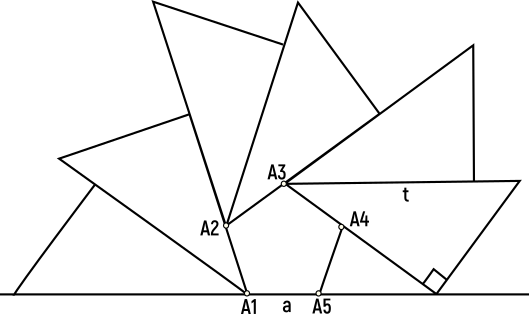
\includegraphics[width=1\linewidth]{1.png} \\ а) макет}
    \end{minipage}
    \hfill
    \begin{minipage}[h]{0.49\linewidth}
    \center{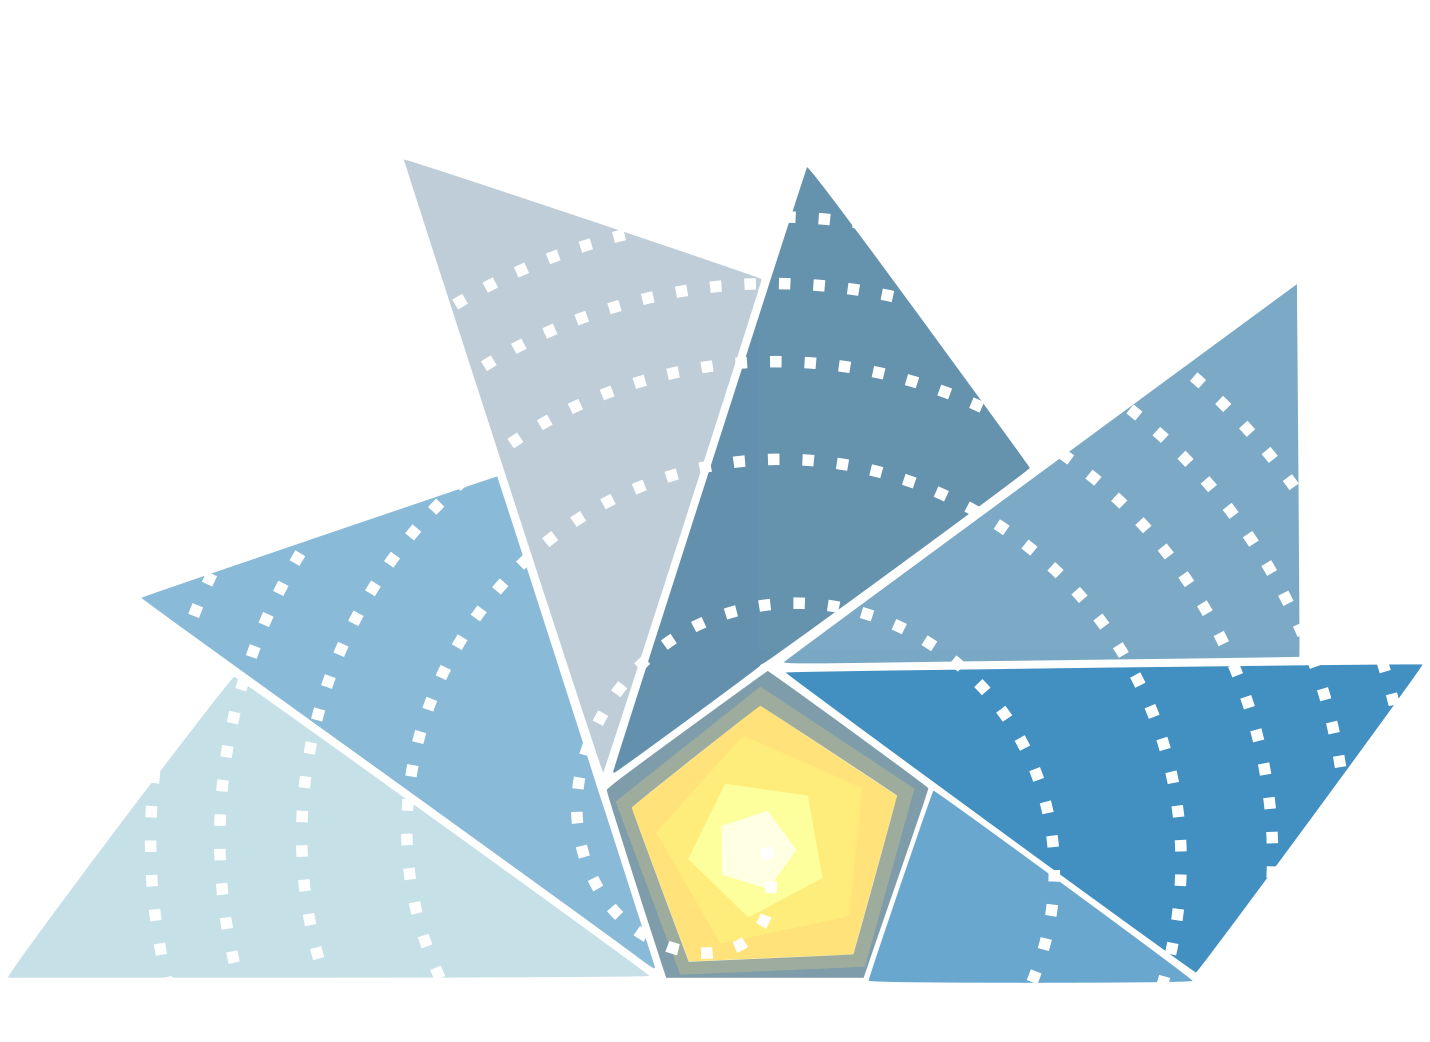
\includegraphics[width=0.9\linewidth]{2.png} \\ б) ожидаемый результат}
    \end{minipage}
\end{figure}

Ворота портала должны быть выполнены ввиде правильного пятиугольника ($A1$, $A2$, $A3$, $A4$, $A1$), из сторон которого выходят “листья” ввиде конгруэнтных  прямоугольных треугольников.

Важно, чтобы результат  точно отображал идею заказчика, поэтому листья не должны заходить за пределы уровня земли. 

Составьте выражения для определения размера гипотенузы треугольника - “листа”,образующего вход в портал.